% VUT FIT MITAI
% MSZ 2021/2022
% Author: Vladimir Dusek
% Login: xdusek27

%%%%%%%%%%%%%%%%%%%%%%%%%%%%%%%%%%%%%%%%%%%%%%%%%%%%%%%%%%%%%%%%%%%%%%%%%%%%%%%%

% Path to figures
\graphicspath{{upa/nosql/figures}}

%%%%%%%%%%%%%%%%%%%%%%%%%%%%%%%%%%%%%%%%%%%%%%%%%%%%%%%%%%%%%%%%%%%%%%%%%%%%%%%%

\chapter{UPA~--~NoSQL databáze (porovnání relačních a NoSQL; CAP věta a ACID/BASE principy; typy NoSQL databází; dotazování v NoSQL databázích; agregace dat pomocí Map-Reduce a agregační pipeline).}

%%%%%%%%%%%%%%%%%%%%%%%%%%%%%%%%%%%%%%%%%%%%%%%%%%%%%%%%%%%%%%%%%%%%%%%%%%%%%%%%

\section{Zdroje}

\begin{compactitem}
    \item \path{09-nosql_databases.pdf}
    \item \path{UPA_2019-11-19.mp4}
    \item \path{szz-kastak.pdf}
    \item \url{https://youtu.be/W2Z7fbCLSTw}
\end{compactitem}

%%%%%%%%%%%%%%%%%%%%%%%%%%%%%%%%%%%%%%%%%%%%%%%%%%%%%%%%%%%%%%%%%%%%%%%%%%%%%%%%

\section{Relační databáze}

\begin{compactitem}
    \item Data organizována do tabulek, řádek reprezentuje záznam (koncept matematické relace, řádek prvkem relace nad doménami sloupcu tabulky).

    \item Každý sloupec má přesně daný (jednoduchý) datový typ (tj. množina/doména odpovídající části relace).

    \item Záznam v tabulce se může odkazovat na záznam (jiné) tabulky (hodnota cizího klíče odpovídá hodnotě primárního klíče odkazovaného záznamu).

    \item Organizace dat musí splňovat normální formy (1NF, 2NF, 3NF, EKNF, BCNF, 4NF, 5NF, DKNF, 6NF1; jinak hrozí redundance/chyby).

    \item Dotazy a úpravy nad daty pomocí SQL (dotazování pomocí SELECT vychází z relační algebry).

    \item Databázový systém zaručuje \textbf{ACID} změnu uložených dat (Atomicity, Consistency, Isolation, Durability). \begin{compactitem}
        \item Jeho zaručení není jednoduché, je třeba provádět a plánovat transakce, řídít souběžný přístup (zamykání), obnovení (rollback), \dots
    \end{compactitem}
\end{compactitem}

\subsection{ACID}

\begin{compactitem}
    \item \textbf{Atomicity} -- Atomičnost transakcí, žádný rozpracovaný stav a to i ve vztahu k možné chybě OS či HW (proběhne celá transakce, tj. všechny její změny, nebo nic).

    \item \textbf{Consistency} -- V DB jsou pouze platná data dle daných pravidel (integritní omezení). Transakce se neuskuteční, pokud to nelze dodržet, jinak platí, že původní i nový stav je platný.

    \item \textbf{Isolation} -- Souběžné transakce se neovlivňují. Serializace. Pořadí však není zajištěno.

    \item \textbf{Durability} -- Uskutečněná transakce nebude ztracena (její projev). Podpora obnovy dat (\textit{rollback}) po pádu HW/SW.
\end{compactitem}

%%%%%%%%%%%%%%%%%%%%%%%%%%%%%%%%%%%%%%%%%%%%%%%%%%%%%%%%%%%%%%%%%%%%%%%%%%%%%%%%

\section{Moderní databáze}

\subsection{Kladené požadavky}

\begin{compactitem}
    \item Cloudová řešení, distribuované databáze: \begin{compactitem}
        \item Decentralizace uložiště dat.
        \item Úmyslná redundance proti výpadkům a pro zajištění rychlosti.
        \item Velké objemy dat a velké množství operací (big data).
    \end{compactitem}

    \item Problematické datové typy: \begin{compactitem}
        \item Údaje klíč-hodnota, objekty, nestrukturované dokumenty, RDF grafy.
    \end{compactitem}

    \item Iterativní vývoj: \begin{compactitem}
        \item Časté změny schématu databáze.
        \item Různé způsoby použití databáze.
    \end{compactitem}

    \item Vysoké požadavky na škálovatelnost: \begin{compactitem}
        \item Mobilní zařízení jako klienti.
        \item Nerovnoměrné rozložení zátěže (prostorové i časové).
        \item Specifické požadavky na dostupnost.
        \item Předem neznámé dotazy, nelze optimalizovat indexy.
    \end{compactitem}
\end{compactitem}

\subsection{Moderní relační databáze}

\begin{compactitem}
    \item Pro uspokojení požadavků na moderní databáze, se zbavujeme relačního modelu a opouštíme předchozí zásady (ACID).

    \item Některé požadavky na moderní databáze není možné uspokojit pouze pomocí rozšíření relačních databází, proto vznikají nová paradigmata.

    \item Dodržování ACID někdy nevhodně omezuje práci s databází, což vede k jeho úmyslnému zanedbání nebo opuštění pro zisk rychlosti a dostupnosti dat.

    \item To má za důsledek vznik specializovaných nerelačních (postrelačních) databází pro strukturovaná data nebo pro specificky přistupovaná data.
\end{compactitem}

\subsection{Co bychom chtěli místo ACID}

\begin{compactitem}
    \item CAP \begin{compactitem}
        \item \textbf{Consistency} -- Každý uzel (každý klient) vidí ve stejný čas stejná data (data jsou konzistentní nezávisle na běžících operacích či jejich umístění).

        \item \textbf{Availability} -- Každý požadavek obsloužen, úspěšně nebo neúspěšně, nepřetržitý provoz (nepřetržitý provoz, vždy možnost číst a zapisovat).

        \item \textbf{Partition tolerance} -- Funkční navzdory chybám sítě nebo výpadkům uzlů.
    \end{compactitem}

    \item Cap věta: \uv{U sdílených (distribuovaných) systémů je možné uspokojit maximálně 2 ze 3 výše uvedených požadavků.}

    \item Proč? \begin{compactitem}
        \item \textbf{Konzistence a dostupnost} -- Databáze není distribuovaná, bude vždy dostupná a konzistentní. To znamená vysokou latenci u vzdálených klientů a také podstatně nižší bezpečnost, riziko výpadku apod.

        \item \textbf{Konzistentní a odolná} -- Databáze distribuovaná na spoustě místech. Aby byla konzistentní, musí se při jakékoliv změně na nějaký okamžik zamknout a počkat až se změny synchronizují. Tím ztratí dočasnou dostupnost.

        \item \textbf{Dostupná a odolná} -- Databáze distribuovaná na spoustě místech, kterou při změně nezamkneme. Synchronizace nějakou dobu trvá. Klient může někdy dostat neaktuální (zastaralá) data.
    \end{compactitem}

    \item Co s tím? \begin{compactitem}
        \item Něco musíme obětovat (řešit jinak), různá řešení pro různé požadavky.

        \item Konzistence a dostupnost -- clusterové databáze, LDAP.

        \item Konzistence a odolnost -- distribuované databáze.

        \item Dostupnost a odolnost -- web caching, DNS.
    \end{compactitem}
\end{compactitem}

%%%%%%%%%%%%%%%%%%%%%%%%%%%%%%%%%%%%%%%%%%%%%%%%%%%%%%%%%%%%%%%%%%%%%%%%%%%%%%%%

\section{NoSQL databáze}

\begin{compactitem}
    \item Nerelační datový model (klíč-hodnota, dokumenty, grafy, \dots) a distribuovaná architektura.

    \item Kdy jsou vhodné? \begin{compactitem}
        \item Pro distribuované uložení či zpracování nerelačních dat.
        \item Pokud potřebujeme vysokou rychlost na úkor ACID.
    \end{compactitem}

    \item Kdy nejsou vhodné? \begin{compactitem}
        \item NoSQL nenahrazují klasické relační databáze, mají jiné využití, pro klasické informační systémy je nejlepší relační databáze.
    \end{compactitem}

    \item NoSQL dodržují tzv. BASE, resp. BaSsEc (CAP s kompromisy), znamená následující: \begin{compactitem}
        \item \textbf{Basically available} -- Většinu času je dostupná. Data nejsou uložena na všech uzlech, jsou rozloženy na některých uzlech s jistým replikačním faktorem (např.: uchováváme tři kopie na nejvíc potřebných místech).

        \item \textbf{Soft-state} -- Databáze může obsahovat neaktuální data a klient s tím musí počítat.

        \item \textbf{Eventual consistency} -- Databáze bude konzistentní po nějaké době (konečný čas).
    \end{compactitem}

    \item Tedy omezuje se konzistence a databáze je vysoce dostupná a odolná proti výpadkům.

    \item Vlastnosti: \begin{compactitem}
        \item Slabá konzistence
        \item 100\,\% dostupnost (dostupná \uv{jak jen to půjde})
        \item Jednodušší a rychlejší
        \item Agresivní, optimistický přístup
        \item Jednodušší evoluce
    \end{compactitem}

    \item Princip NoSQL paradigmat: \begin{compactitem}
        \item Několik typů databází, většina založena na principu klíč-hodnota.
        \item Implementováno pomocí hashování (extrémně rychlé).
        \item Hodnota je BLOB (binary large object) -- databáze se je často vůbec nesnaží chápat.
        \item Nemá předdefinované schéma -- flexibilita.
        \item Vysoká škálovatelnost (přidávání, ubírání dat).
        \item Pokud nás zajímá pouze část hodnoty, ať pro dotazy nebo zápis, tak je poměrně neefektivní.
    \end{compactitem}

    \item Podpora \textit{partitioning} (\textit{sharding}) -- Rozdělení dat na různé uzly v clusteru.
\end{compactitem}

\begin{figure}[H]
    \centering
    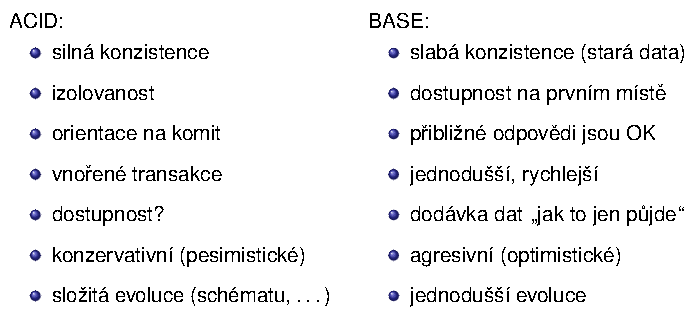
\includegraphics[width=1\linewidth]{acid-vs-base.pdf}
    \caption{Porovnání ACID vs BASE.}
\end{figure}

\subsection{Jednotlivá NoSQL paradigmata}

\subsubsection*{Key-value databáze}

\begin{compactitem}
    \item Databáze key-value je jednoduché paradigma ukládání, načítání a správu dat ve formátu key-value (podobná struktura jako Python slovník, nebo JSON).
    \item Nevyhodnocují se žádné \textit{queries} ani \textit{joins}.
    \item Extrémně rychlé, jelikož všechna data jsou držena v paměti.
    \item Využití: \begin{compactitem}
        \item jako cache nad jinou datovou vrstvou,
        \item jako message broker (např. Celery, systém pro správu distribuované fronty úloh).
    \end{compactitem}
    \item Např. Redis, Memcached, Oracle NoSQL, \dots
\end{compactitem}

\subsubsection*{Sloupcové databáze (\textit{wide column})}

\begin{compactitem}
    \item Řádky jako u relační databáze, u řádků máme různé sloupce s hodnotami, ale narozdíl od relačních databází nemá schéma (ačkoliv data jsou svým způsobem strukturovaná).
    \item Klíč-hodnota, kde hodnota je řádek v tabulce.
    \item Optimalizované pro čtení dat po sloupcích, místo po řádcích (vhodné pro analýzu).
    \item Dotazovací jazyk podobný SQL (nemá \textit{joins}).
    \item Využití: \begin{compactitem}
        \item škálování velké množství time-series dat (záznamy z IoT zařízení, senzorů, \dots),
        \item pro historická data,
        \item high-write, low-read.
    \end{compactitem}
    \item Např. Apache Cassandra, Apache HBase (Google Bigtable), \dots
\end{compactitem}

\subsubsection*{Dokumentové databáze (\textit{document oriented})}

\begin{compactitem}
    \item Nestrukturované dokumenty (bez schéma), každý dokument ve formátu key-value.
    \item Dokumenty mohou být seskupovány do kolekcí, kolekce mají indexy a mohou být organizovány do hierarchie.
    \item Nepodporují joiny.
    \item Využití: \begin{compactitem}
        \item mobilní hry,
        \item IoT,
        \item obecně aplikace,
        \item celkově široké využití.
    \end{compactitem}
    \item Např. MongoDB, Firestore, \dots
\end{compactitem}

% MongoDB dokument oriented
% stored in binary json in collections (optional)
% flexible schema
% extreme fast reading (no joins)

\subsubsection*{Grafové databáze}

\begin{compactitem}
    \item Alternativa k relačním databázím.
    \item Uchováváme uzly a hrany, které tyto uzly spojují.
    \item Využití: \begin{compactitem}
        \item RDF dokumenty,
        \item Reprezentace sítí (dopravní, počítačové) a jejich topologie.
    \end{compactitem}
    \item Např. Neo4j, Dgraph, \dots
\end{compactitem}

\subsection{Dotazování v NoSQL}

\begin{compactitem}
    \item Klíč se využívá na: \begin{compactitem}
        \item Nalezení správného uzlu v clusteru pro daný klíč (pomocí directory service a nebo distribuované hashovací tabulky).

        \item Následně nalezení diskového bloku, kde je hodnota uložena v rámci uzlu (pomocí stromových struktur, hashovací tabulky, \dots).
    \end{compactitem}

    \item Je těžké vykonávat nad dotazi nějaké optimalizace (jako se děje v relačních databází).

    \item Typicky není podporována \textit{join} operace.

    \item Filtrování podle klíče: \begin{compactitem}
        \item Vždy podporováno.
        \item Klíč je primární index, implementovaný pomocí distribuované hashovací tabulky.
        \item Je možné zavést druhořadé indexy, pouze pro dotazování (ne pro \textit{sharding}).
    \end{compactitem}

    \item Filtrování podle hodnoty: \begin{compactitem}
        \item Podporované pouze ve specializovaných NoSQL.
    \end{compactitem}
\end{compactitem}

\subsection{Agregace dat}

% todo: lepe

\begin{compactitem}
    \item Agregace $\sim$ \textit{grouping}.
    \item Je omezené hranicemi daného shardu (je snažší agregovat data v rámci shardu).
    \item Map-Reduce se používá pro složité nebo vlastní agregace.

    \item \textbf{Agregace pomocí Map-Reduce} \begin{compactitem}
        \item Ve fázi \textit{map} se odděleně vykoná daná operace \textit{map} na dataset na každém uzlu (transformace vstupní kolekce na výstupní).
        \item Výsledky operace \textit{map} ze všech uzlů, se podle klíče spojí dohromady (tzv. \textit{handshake} fáze pro výměnu dat mezi uzly).
        \item Nakonec se podle jednotlivých hodnot klíče aplikuje zadaná \textit{reduce} operace na každý seznam hodnot.
    \end{compactitem}

    \item \textbf{Agregační pipeline} \begin{compactitem}
        \item V MongoDB.
        \item Dokumenty vstupují do více úrovňové pipeline, která je transformuje na výsledek.
        \item Jde o pipeline pro zpracování a hlavní agregaci a filtrování dat (agregační vzory).
        \item Všechny výsledky, průběžné i finální, jsou kolekce dokumentů.
    \end{compactitem}
\end{compactitem}
